\documentclass{article}

\usepackage{mathtools,amsfonts,amssymb}
\usepackage{enumerate}
\usepackage{fullpage}
\usepackage{fancyvrb}


\begin{document}
\thispagestyle{empty}

\begin{center}
  \textbf{\Large Intermediate Test 1 Solutions}
  % LEVEL is Senior, Intermediate or Beginner
  % NUMBER is the test number: 1, 2, etc.
  \\ \vspace{1em}
  \textbf{\large January Camp 2021}
  \\ \vspace{1em}
  \textbf{\large Time: $2\frac{1}{2}$ hours}
\end{center}

\vspace{24pt}

\begin{enumerate}[1.]

\item {\itshape You are given the following shape: % South Africa, Tim's Assorted Combinatorics Questions 2020, Q2
	\begin{center}
	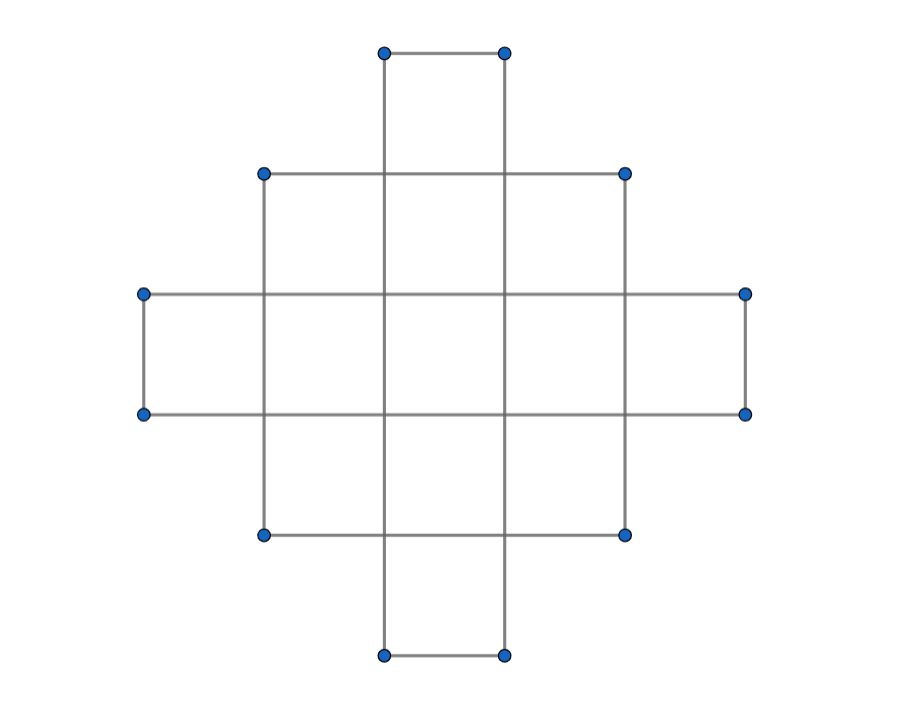
\includegraphics[scale=0.3]{Capture.png}	
	\end{center}
You need to tile this with L-shapes made of 3 blocks. Which single blocks could you shade out of the original diagram to make this possible? }

Note that any L-block covers at most 1 shaded square. To cover all of them, we would need 5 L-blocks, covering a total of 15 squares, when we only have 13 squares. So without removing one of these, we will not be able to tile the image. On the other hand, removing one of these squares always results in a possible tiling. This is left as an exercise.

\item % Ukraine 2016-2017, Third Round 2017, First Tour, 4.1
{\itshape Let $ABCD$ be a trapezoid with $AD \parallel BC$. The angle bisector of $\angle DAB$ intersects the angle bisectors of $\angle ABC$ and $\angle CDA$ at points $P$ and $S$ respectively, and the angle bisector of $\angle BCD$ intersects the angle bisectors of $\angle ABC$ and $\angle CDA$ at points $Q$ and $R$ respectively. Furthermore, $PS \parallel RQ$. Prove that $AB = CD$. }

Extend $CQ$ onto $AD$. Let $T$ be the intersection of $CQ$ and side $AD$.  Since we have $AD \parallel BC$, $\angle DTC = \angle QCB$ with alternating angles. 
Also, since $PS \parallel QR$, we also have corresponding angles $\angle DAP = \angle DTC \implies \angle DAP = \angle QCB$. We now have $\angle BAD = 2\cdot \angle DAP = 2\cdot \angle QCB = \angle BCD$. Since the opposite angles of the trapezoid are now equal, we know this trapezoid is a parallelogram. Since the opposite sides of a parallelogram are equal in length, we will have $AB = CD$.
%can add alternate solution

\item % Moldova, 61st Maths Olympiad (2017), 7.1 modified
{\itshape Find all natural numbers $x$, $y$ and $z$ satisfying 
$$x + \frac{1}{y + \frac{1}{z}} = \frac{850862}{421}$$}

Note $\frac{850862}{421}$ = $2021\frac{21}{421}$ where 2021 is the integer part of the fraction.

Since $y$ and $z$ are given as natural numbers, we have that $y + \frac{1}{z} > 1$ which implies $\frac{1}{y + \frac{1}{z}} < 1$. Since $x$ is a natural number,  $\frac{1}{y + \frac{1}{z}}$ will need to be the fractional part of  $2021\frac{21}{421}$. This will make $x$ the integer part of $2021\frac{21}{421}$ which means $x$ = 2021. Now we are left with $\frac{1}{y + \frac{1}{z}} = \frac{21}{421}$ which we can rewrite as $y + \frac{1}{z} = \frac{421}{21} = 20\frac{1}{21}$. Since $z\geq1$, we will have $\frac{1}{z}\leq1$. If $z = 1$, $y + \frac{1}{z} = y + \frac{1}{1} = y + 1 = 20\frac{1}{21}$ which would make $y = 19\frac{1}{21}$. This would be a contradiction since $y$ is given as a natural number. From this we conclude that $z\neq 1$ and that $\frac{1}{z}<1$ . This means that $\frac{1}{z}$ will be the fractional part and $y$ the integer part of $20\frac{1}{21}$. This makes $y = 20$ and $z = 21$. 
This means the only possible solution for $(x, y, z)$ is $(2021, 20, 21)$. 

\item % Ukraine 2018-2019, 3rd round, second tour, 9th Grade, Q1
{\itshape Find all possible real numbers $k$ such that the values of $x$ satisfying
$$k(2 - k)x^2 - (k + 4)x + 6 = 0$$
are positive integers.}

Firstly, notice that if $k(2 - k) = 0$, then $x = \frac{6}{k + 4}$. The only positive integer solution of this is when $k = 2$: $x = 1$.
Assuming $k(2 - k) \ne 0$, we can use the quadratic formula. We see that the solutions of the equation in $x$ are
\begin{align*}
    x &= \frac{(k + 4) \pm \sqrt{(k + 4)^2 - 24k(2 - k)}}{2k(2 - k)} \\
    &= \frac{(k + 4) \pm \sqrt{25k^2 - 40k + 16}}{2k(2 - k)} \\
    &= \frac{(k + 4) \pm \sqrt{(5k - 4)^2}}{2k(2 - k)} \\
    &= \frac{(k + 4) \pm (5k - 4)}{2k(2 - k)}
\end{align*}
The two solutions are thus $x_1 = \frac{6k}{2k(2 - k)} = \frac{3}{2 - k}$ and $x_2 = \frac{8 - 4k}{2k(2 - k)} = \frac{2}{k}$. Now we must have that $\frac{2}{k}$ and $\frac{3}{2 - k}$ are integers simultaneously. $\frac{2}{k} \in \mathbb{Z} \iff k = \frac{2}{n}$ where $n \in \mathbb{Z}$. Hence we must have the following is an integer 
$$\frac{3}{2 - k} = \frac{3}{2 - \frac{2}{n}} = \frac{3n}{2n - 2}= \frac{3n}{2(n - 1)}$$

Having $n - 1 | 3$ yields $n \in \{-2, 0, 2, 4\}$. If $n - 1 \nmid 3$, we must have $2(n - 1) | n$. If $n > 2$, then $2(n - 1) > n$. If $n < 0$, then $2(n - 1) < n < 0$. Thus we only need to check $n \in \{0, 1, 2\}$. The values of $k$ that we get are $k \in \{-1, 1, \frac{1}{2}, 2\}$. It can then be checked that the only $k$ values that provide positive integers solutions are 
$$k \in \{\frac{1}{2}, 1, 2\}$$

\item % Ireland, 2017, Powerful Sequences, Q2
{\itshape Let $O$ be the circumcentre of $\triangle ABC$. Let $X$, $Y$ and $Z$ be the reflections of $O$ over $BC$, $CA$ and $AB$ respectively. Prove that $\triangle XYZ$ is congruent to $\triangle ABC$ and the corresponding sides are parallel.}

Let $X'$ be the intersection of $OX$ and $BC$ and $Z'$ be the intersection of $OZ$ and $AB$. Since $X$ is the reflection of $O$ across $BC$ we have $OX' = X'X$ as well as $OX \perp BC$ and since $X'$ is on $OX$ we also have $OX' \perp BC$. $BC$ is a chord on the circumcircle with centre $O$ and $OX'$ is a perpendicular on $BC$, thus $BX' = X'C$. By similar arguments we have $OZ' = Z'Z$ and $AZ' = Z'B$. 

By midpoint theorem on $\triangle ABC$, we have $X'Z'||CA$ and $2XX' = AC$. By midpoint theorem on $\triangle OZX$, we have $X'Z'||XZ$ and $2X'Z' = XZ$. Therefore, $XZ||X'Z'||CA$ and $XZ = 2X'Z' = AC$. Applying similar arguments to prove $XY = AB$, and $YZ = BC$ gives $\triangle ABC \equiv \triangle XYZ$. The correspoonding sides are parallel part follows with similar arguments as well. 



\end{enumerate}


\vfill
% ASCII art
\centering
\begin{BVerbatim}
      ,~~.
     (  6 )-_,
(\___ )=='-'
 \ .   ) )
  \ `-' /    
~'`~'`~'`~'`~
\end{BVerbatim}

\end{document}
